%
% Kapitel1.tex
%
%
\chapter{Introduction}
Perimeter Monitoring is one of the most important elements which serves as the useful element in security and surveillance of a location. This thesis employs Digital Acoustic Sensing (DAS)~\cite{duckworth}, configuring it to detect various activities. The activities walking, intrusion detection, gate monitoring and other climbing activities serve as baseline for a perimeter monitoring system. In this thesis the focus is on the detection of different walking patterns and footsteps. Once the system detects the walking pattern, the approach integrates additional activities to complete the system. The proposed solution deploys the system in various perimeters such as borders, national parks, airports, and more.

\begin{figure}[h]
    \centering
    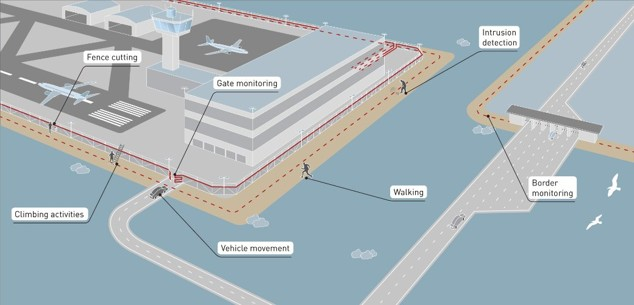
\includegraphics[width=\linewidth]{Bilder/jpg/Airport.jpg}
    \caption{Perimeter Monitoring System at Airport~\cite{Airport_Image}}
    \label{Airport}
\end{figure}

The Figure~\ref{Airport} shows the cable layout for the perimeter monitoring that serves as a baseline plan for deployment on the airport. There are various activities in the picture like walking, climbing, vehicle movement as discussed above. The DAS system detects all these activities by running an algorithm that filters and identifies them. The setup connects the DAS system to the fibre optic cable, as indicated by the red lines in Figure \ref{Airport}.

\begin{figure}[h]
    \centering
    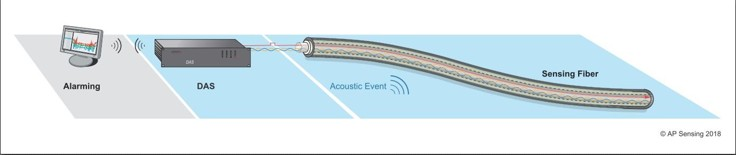
\includegraphics[width=\linewidth]{Bilder/jpg/System.jpg}
    \caption{DAS Setup~\cite{DAS_PPT}}
    \label{System}
\end{figure}

The DAS system has a fibre optic cable which is one big sensor used for detecting distortions. It operates like a long chain of highly sensitive microphones which provides accurate measurements of the acoustic field by giving out amplitude, frequency and phase which has true linearity over distance, time and acoustic intensity. AP Sensing developed DAS system is used in this thesis. AP Sensing developed the DAS Configurator application, which serves to access the DAS system via the network. The IP address of the specific DAS system can be added to it. Figure~\ref{System} shows how the different elements in the DAS system are connected. A computer accesses all the data that DAS collects along the fibre optic cable, and the system applies various algorithms to detect different activities. The system triggers an alarm when it detects a particular activity.

This thesis focuses on various algorithms developed for footsteps detection which will lead to the detection of walking. The detection uses threshold values and various other pattern detection methods with the help of deep learning models such as ConvNext V2 \cite{liu2023convnextv2} and EfficientNet \cite{tan2019efficientnet}. The study evaluates these models and methods for walking detection by training them on the same dataset. The study determines the best model by evaluating its real-time performance.
